\vphantom{loh}\\
\vphantom{loh}\\
\section{MSE-Headless-AD In-Context Curves on Bernoulli Bandit}
\label{appendix:mse_headless_curves}

% \hphantom{loh}

\begin{figure*}[!h]
    \vskip 0.2in
    \centering
    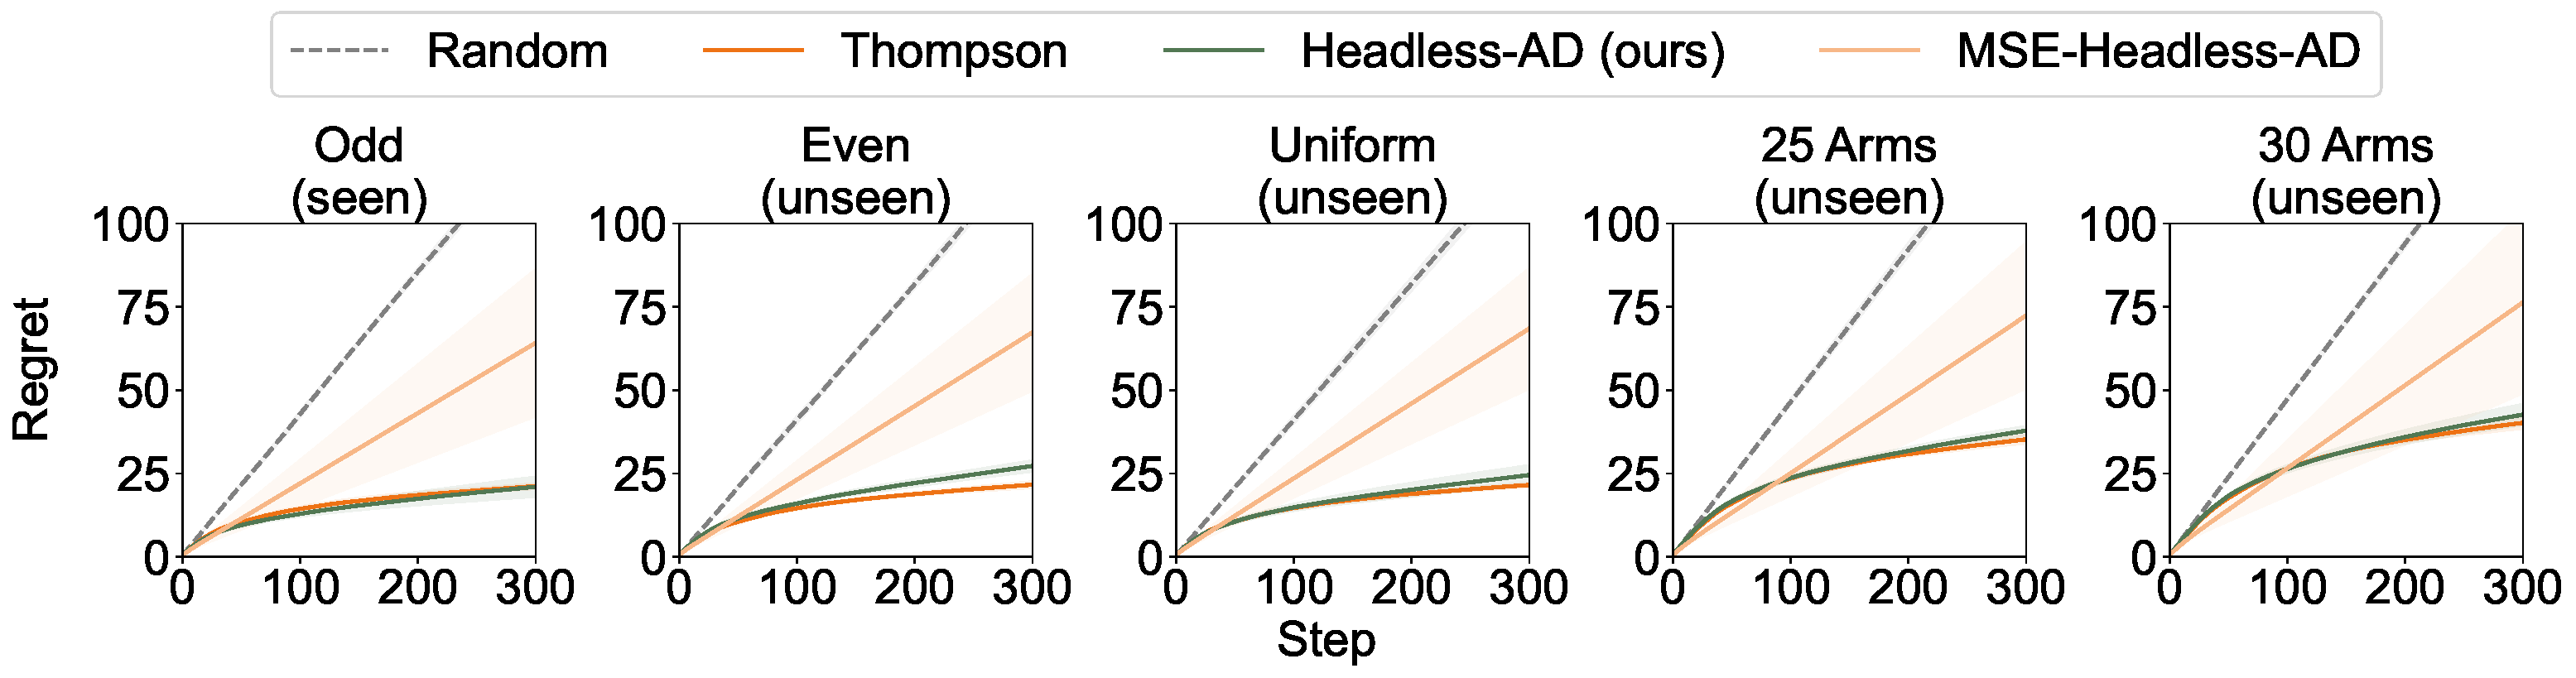
\includegraphics[width=0.9\textwidth]{images/bandit_vanilla_mse.pdf}
    \caption{\textbf{MSE-Headless-AD In-Context Curves on Benroulli Bandit:} Though \Cref{table:ablations} shows that a variant of Headless-AD with MSE loss has a far from random regret, this graph shows that this result is due to the exploitation of several actions and the lack of exploration. We make this conclusion by observing that the shape of MSE-Headless-AD's training curve is a straight line, showing the evidence that no learning is being present. All curves are averaged over $5$ seeds.}
    \label{fig:mse_headless_curves}
    \vskip -0.2in
\end{figure*}
